\section{Introdução} \bigskip
Nos dias de hoje, o voluntariado é cada vez mais praticado na nossa sociedade. Segundo um estudo realizado pelo INE - Instituto Nacional de Estatística, em 2019, cerca de 6,4\% da população portuguesa realiza trabalho voluntário, uma percentagem que cresceu ligeiramente face aos resultados obtidos em 2012 $(5,9\%)^{[1]}$.
\par \bigskip

O trabalho voluntário, ou voluntariado, segundo o diário da república, tem como definição: \par \bigskip

\textit{
	``O conjunto de ações de interesse social e comunitário realizadas de forma desinteressada por pessoas, no âmbito de projetos, programas e outras formas de intervenção ao serviço dos indivíduos, das famílias e da comunidade desenvolvidos sem fins lucrativos por entidades públicas ou privadas.``$^{[2]}$
} \par \bigskip

Esta definição entrega ao voluntário (quem realiza voluntariado) o papel fulcral na sociedade de tentar enriquecer a mesma sem qualquer contrapartida. A participação em ações de voluntariado permite a obtenção de competências multi-disciplinares que são valorizadas no mundo profissional, e como tal, cada vez mais empresas dão valor a candidatos que participam nestas ações. \par \bigskip

Atualmente, a candidatura ao voluntariado é efetuada através de múltiplas plataformas, como redes sociais e \textit{websites}, algo que descentraliza estes serviços porque cada organização usa o seu próprio modelo.

\bigskip \bigskip \bigskip 

\begin{figure}[h]
	\centering
	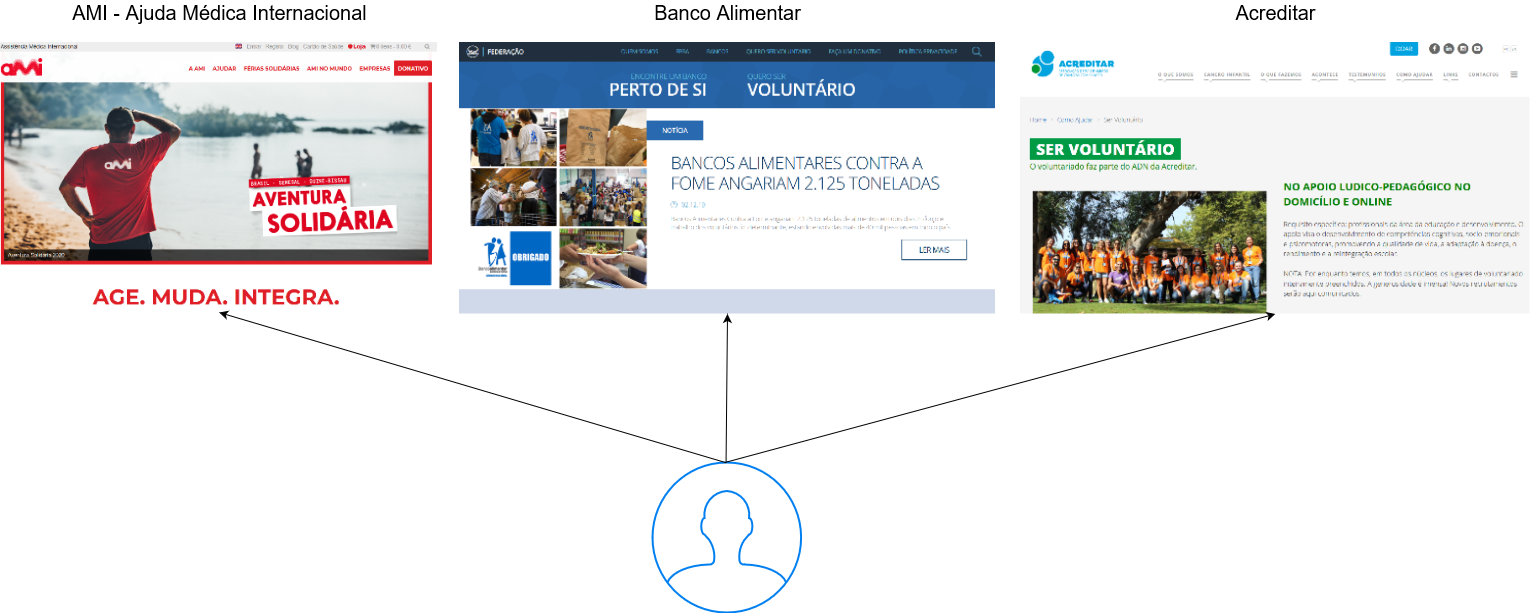
\includegraphics[scale=0.20]{services-decentralized}
	\caption{Modelo descentralizado de divulgação de voluntariado}	
\end{figure}

\newpage

O nosso projeto tem como objetivo desenvolver uma "rede social" \space com foco no voluntariado, sendo uma plataforma que irá disponibilizar às entidades organizadoras a possibilidade de divulgar e organizar estas ações, e aos voluntários, serviços que facilitam aos mesmos manterem-se informados e participarem nas mesmas.

\bigskip \bigskip \bigskip

\begin{figure}[h]
	\centering
	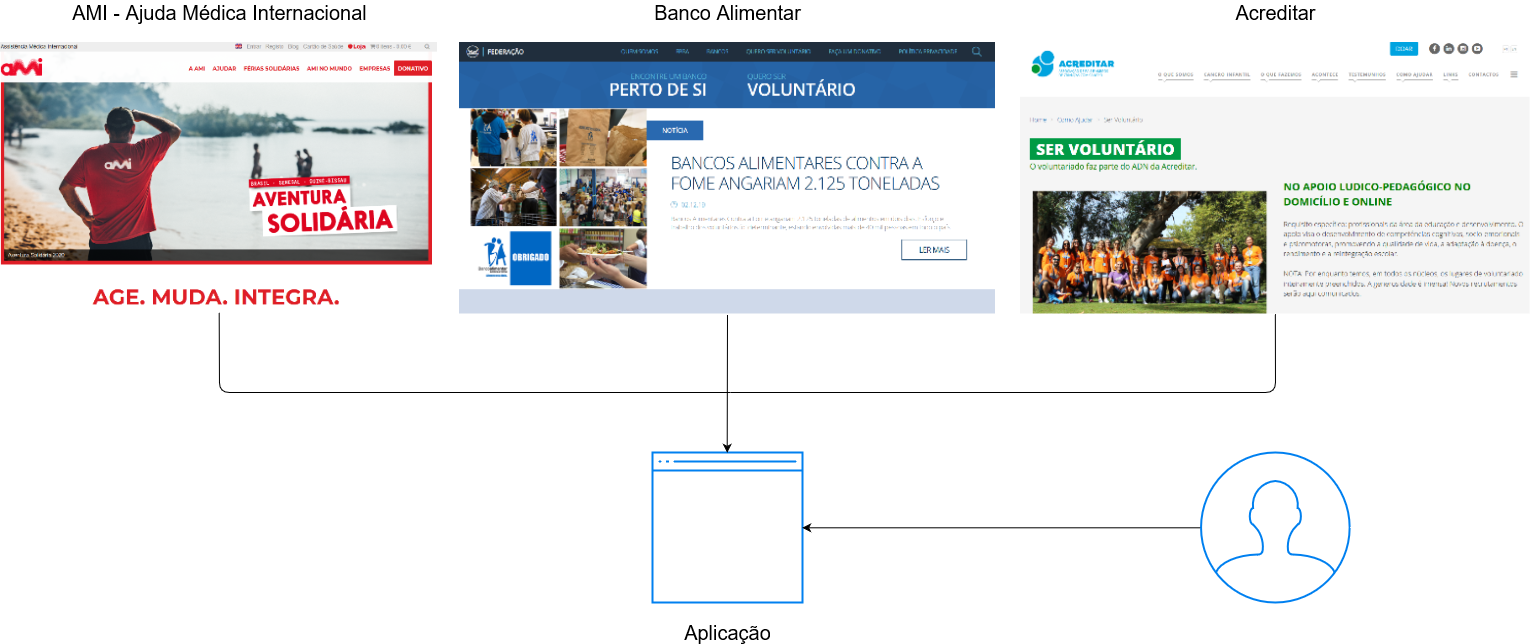
\includegraphics[scale=0.20]{services-centralized}
	\caption{Conceito do projeto}
\end{figure}